\renewcommand{\slideid}{L3-PY10}
\begin{frame}[c]{Python lab 5: infer a coefficient from sparse data}
\small
\[
 -\kappa u''=\pi^2\sin(\pi x),\qquad u(0)=u(1)=0,
 \qquad \text{true }\kappa=0.7.
\]
\lstinputlisting[style=pythonlab]{experiments/snippets/inverse_loss.py}
\begin{block}{A synthetic inverse problem}
\InverseDataProtocol. The network and $\kappa$ are trained jointly.
\end{block}
\labnote{\InverseTrainProtocol.}
\end{frame}

\renewcommand{\slideid}{L3-PY11}
\begin{frame}[c]{Python output: recover a field and its coefficient}
\small
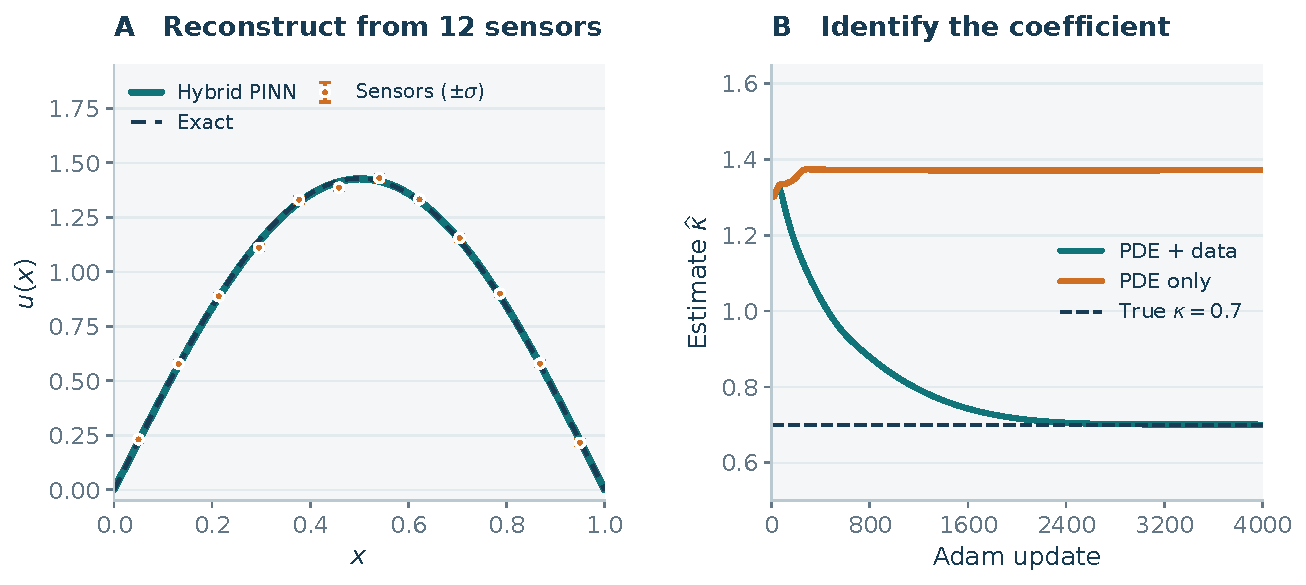
\includegraphics[width=\textwidth]{experiments/figures/inverse_recovery.pdf}
\begin{block}{Results for this noise realization}
Learned $\widehat\kappa=\textbf{\InverseKappa}$ (truth $0.7$);
coefficient error \textbf{\InverseKappaError}.
Relative field $L^2$ error: \textbf{\InverseLtwo}.
\end{block}
\labnote{The coefficient curve shows Adam iterations; the final values include
L-BFGS refinement. Noise level and optimizer settings are recorded with the results.}
\end{frame}

\renewcommand{\slideid}{L3-PY12}
\begin{frame}[c]{Python output: why the observations are essential}
\small
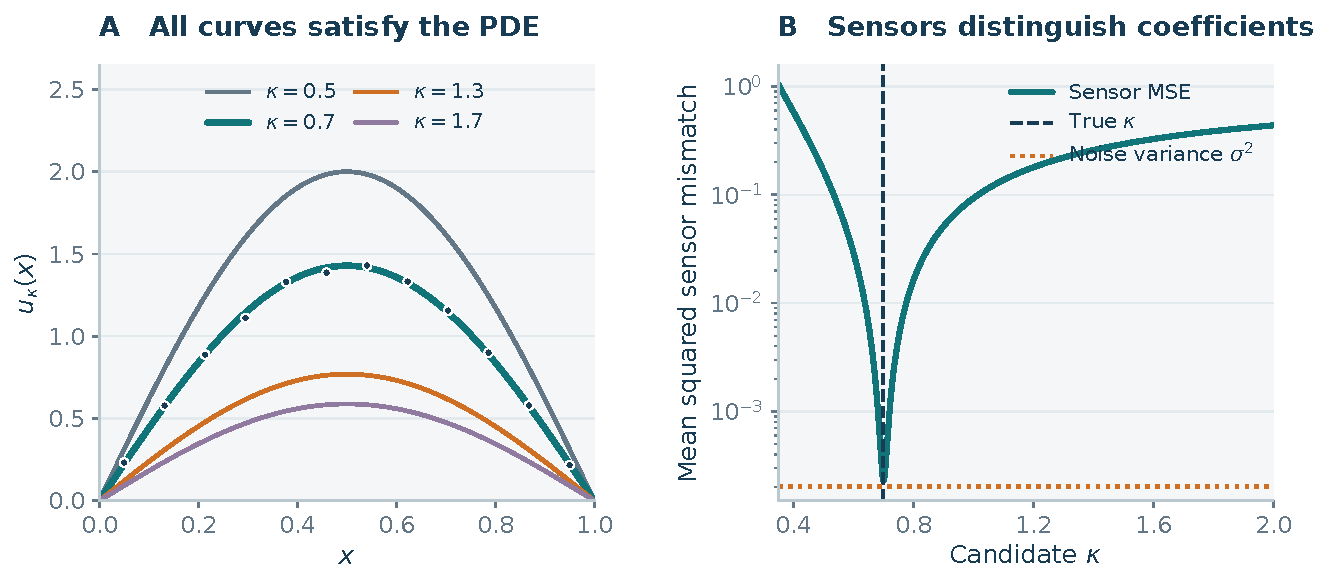
\includegraphics[width=\textwidth]{experiments/figures/inverse_identifiability.pdf}
\begin{block}{The PDE and boundary data leave a family of solutions}
For every $\kappa>0$, $u_\kappa(x)=\sin(\pi x)/\kappa$ solves the PDE.
Interior observations select a coefficient within this family.
\end{block}
\labnote{The right panel evaluates the analytic solution family at the noisy
sensors to show which coefficients fit the observations.}
\end{frame}
\renewcommand{\slideid}{L3}
